\documentclass[10pt, conference, a4paper, final]{IEEEtran}
\IEEEoverridecommandlockouts
\usepackage{amsmath, amssymb}
\usepackage[margin=1in]{geometry} % Adjust margins if needed
\usepackage{graphicx} % Required for including images
\usepackage{subcaption}
\usepackage{algorithm, algorithmicx} % For algorithms
\usepackage[table,xcdraw]{xcolor} % For colored tables
\usepackage{enumitem} % For better control over list
\usepackage{microtype} % Improves typography

% Combine graphicx package loading
\usepackage{float}
\usepackage{booktabs} % For professional looking tables

\title{Local and Global Coverage Assessment of Deep Learning Models}
\author{Author Name}
\date{\today}

\begin{document}

\maketitle

\begin{abstract}
% Your abstract goes here.
\end{abstract}


\section{Introduction}
\begin{itemize}[noitemsep]
    \item Background
    \item Generic problem
    \item Existing solution
    \item Problem in existing solutions
\end{itemize}

\section{Methodology}
\begin{figure*}{H}
    \centering
    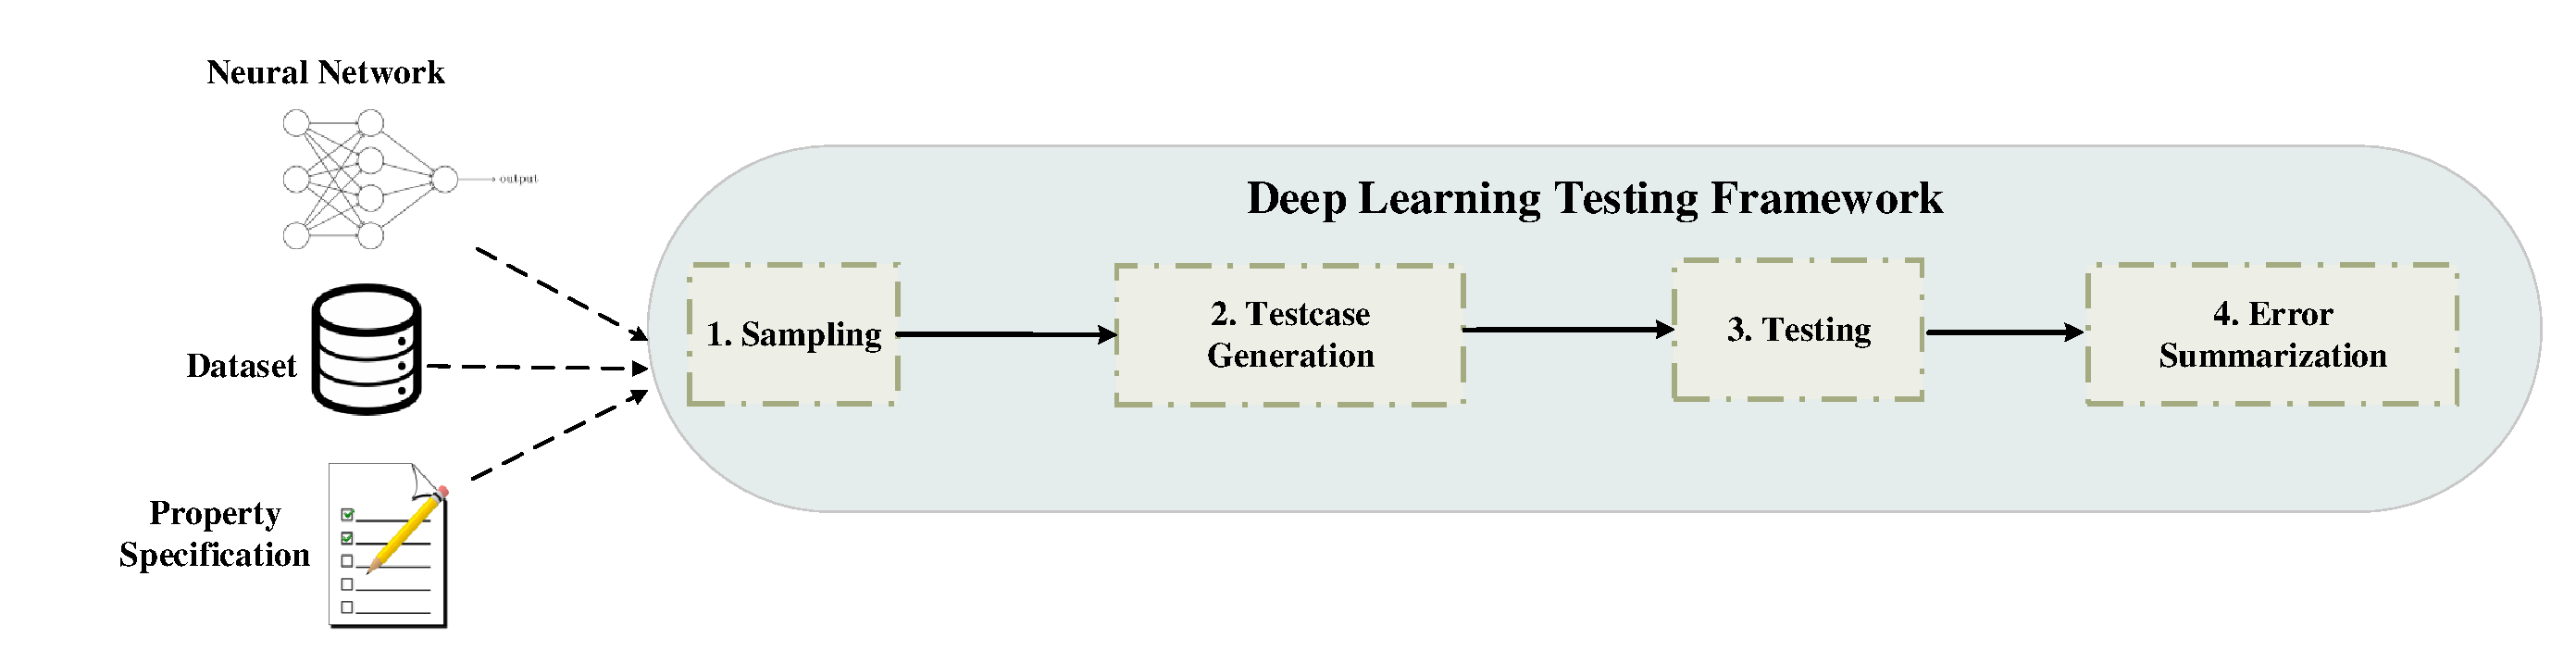
\includegraphics[width=\linewidth]{paper_images/DL framework.pdf}
    \caption{Graphical Representation}
    \label{fig:graph}
\end{figure*}
\subsection {Define Criteria}
\subsection {Sampling}
\subsection {Test Case Generation}
\subsection {Verify Test Cases}
\subsection {Probabilistic Graph}
\subsection {Feedback}
% Attempt to include figures compactly
% \begin{figure}[H]
%     \centering
%     \begin{subfigure}{.5\textwidth}
%         \centering
%         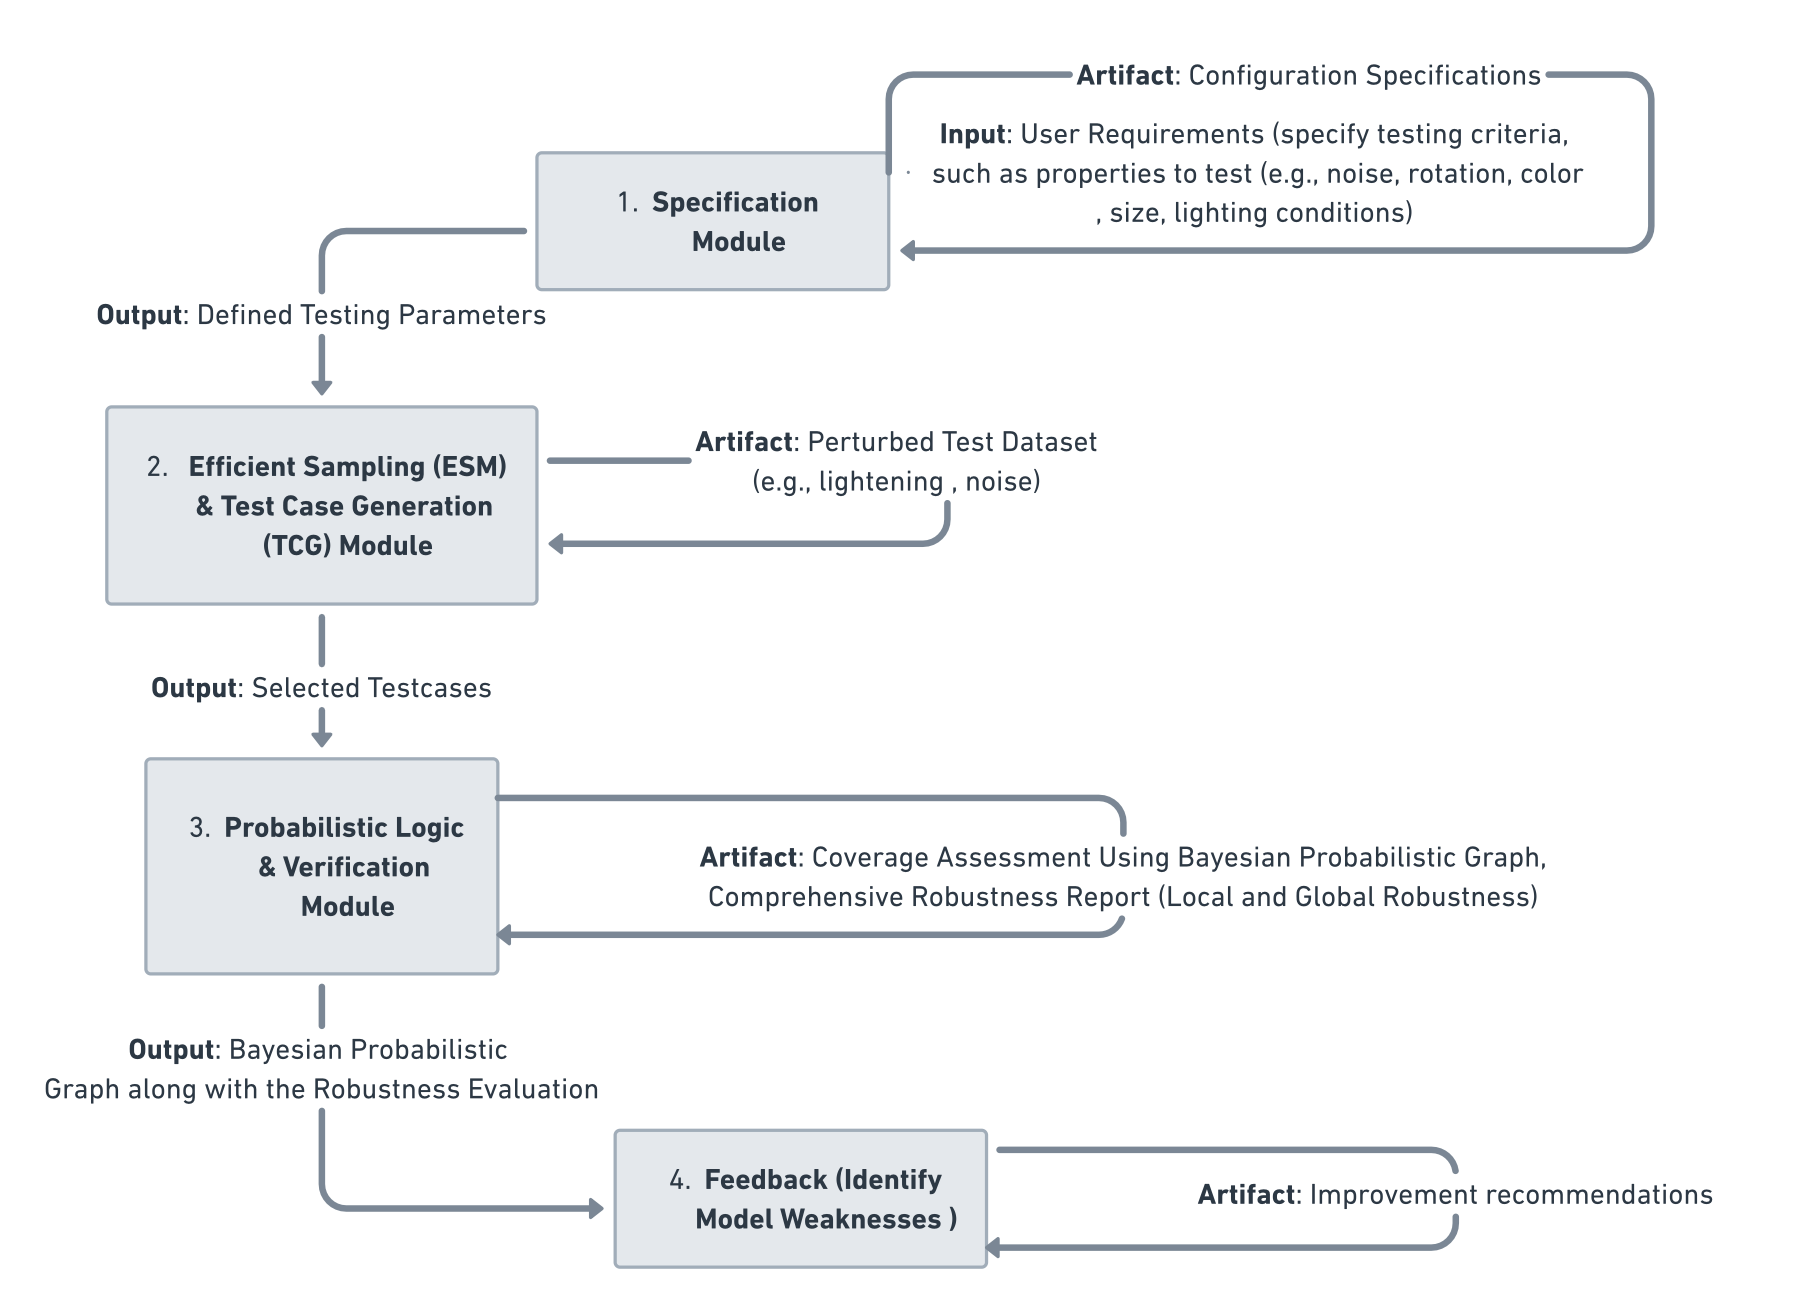
\includegraphics[width=\linewidth]{paper_images/overview.png}
%         \caption{Model Overview}
%         \label{fig:overview}
%     \end{subfigure}%
  
% \end{figure}

\begin{figure*}{H}
    \centering
    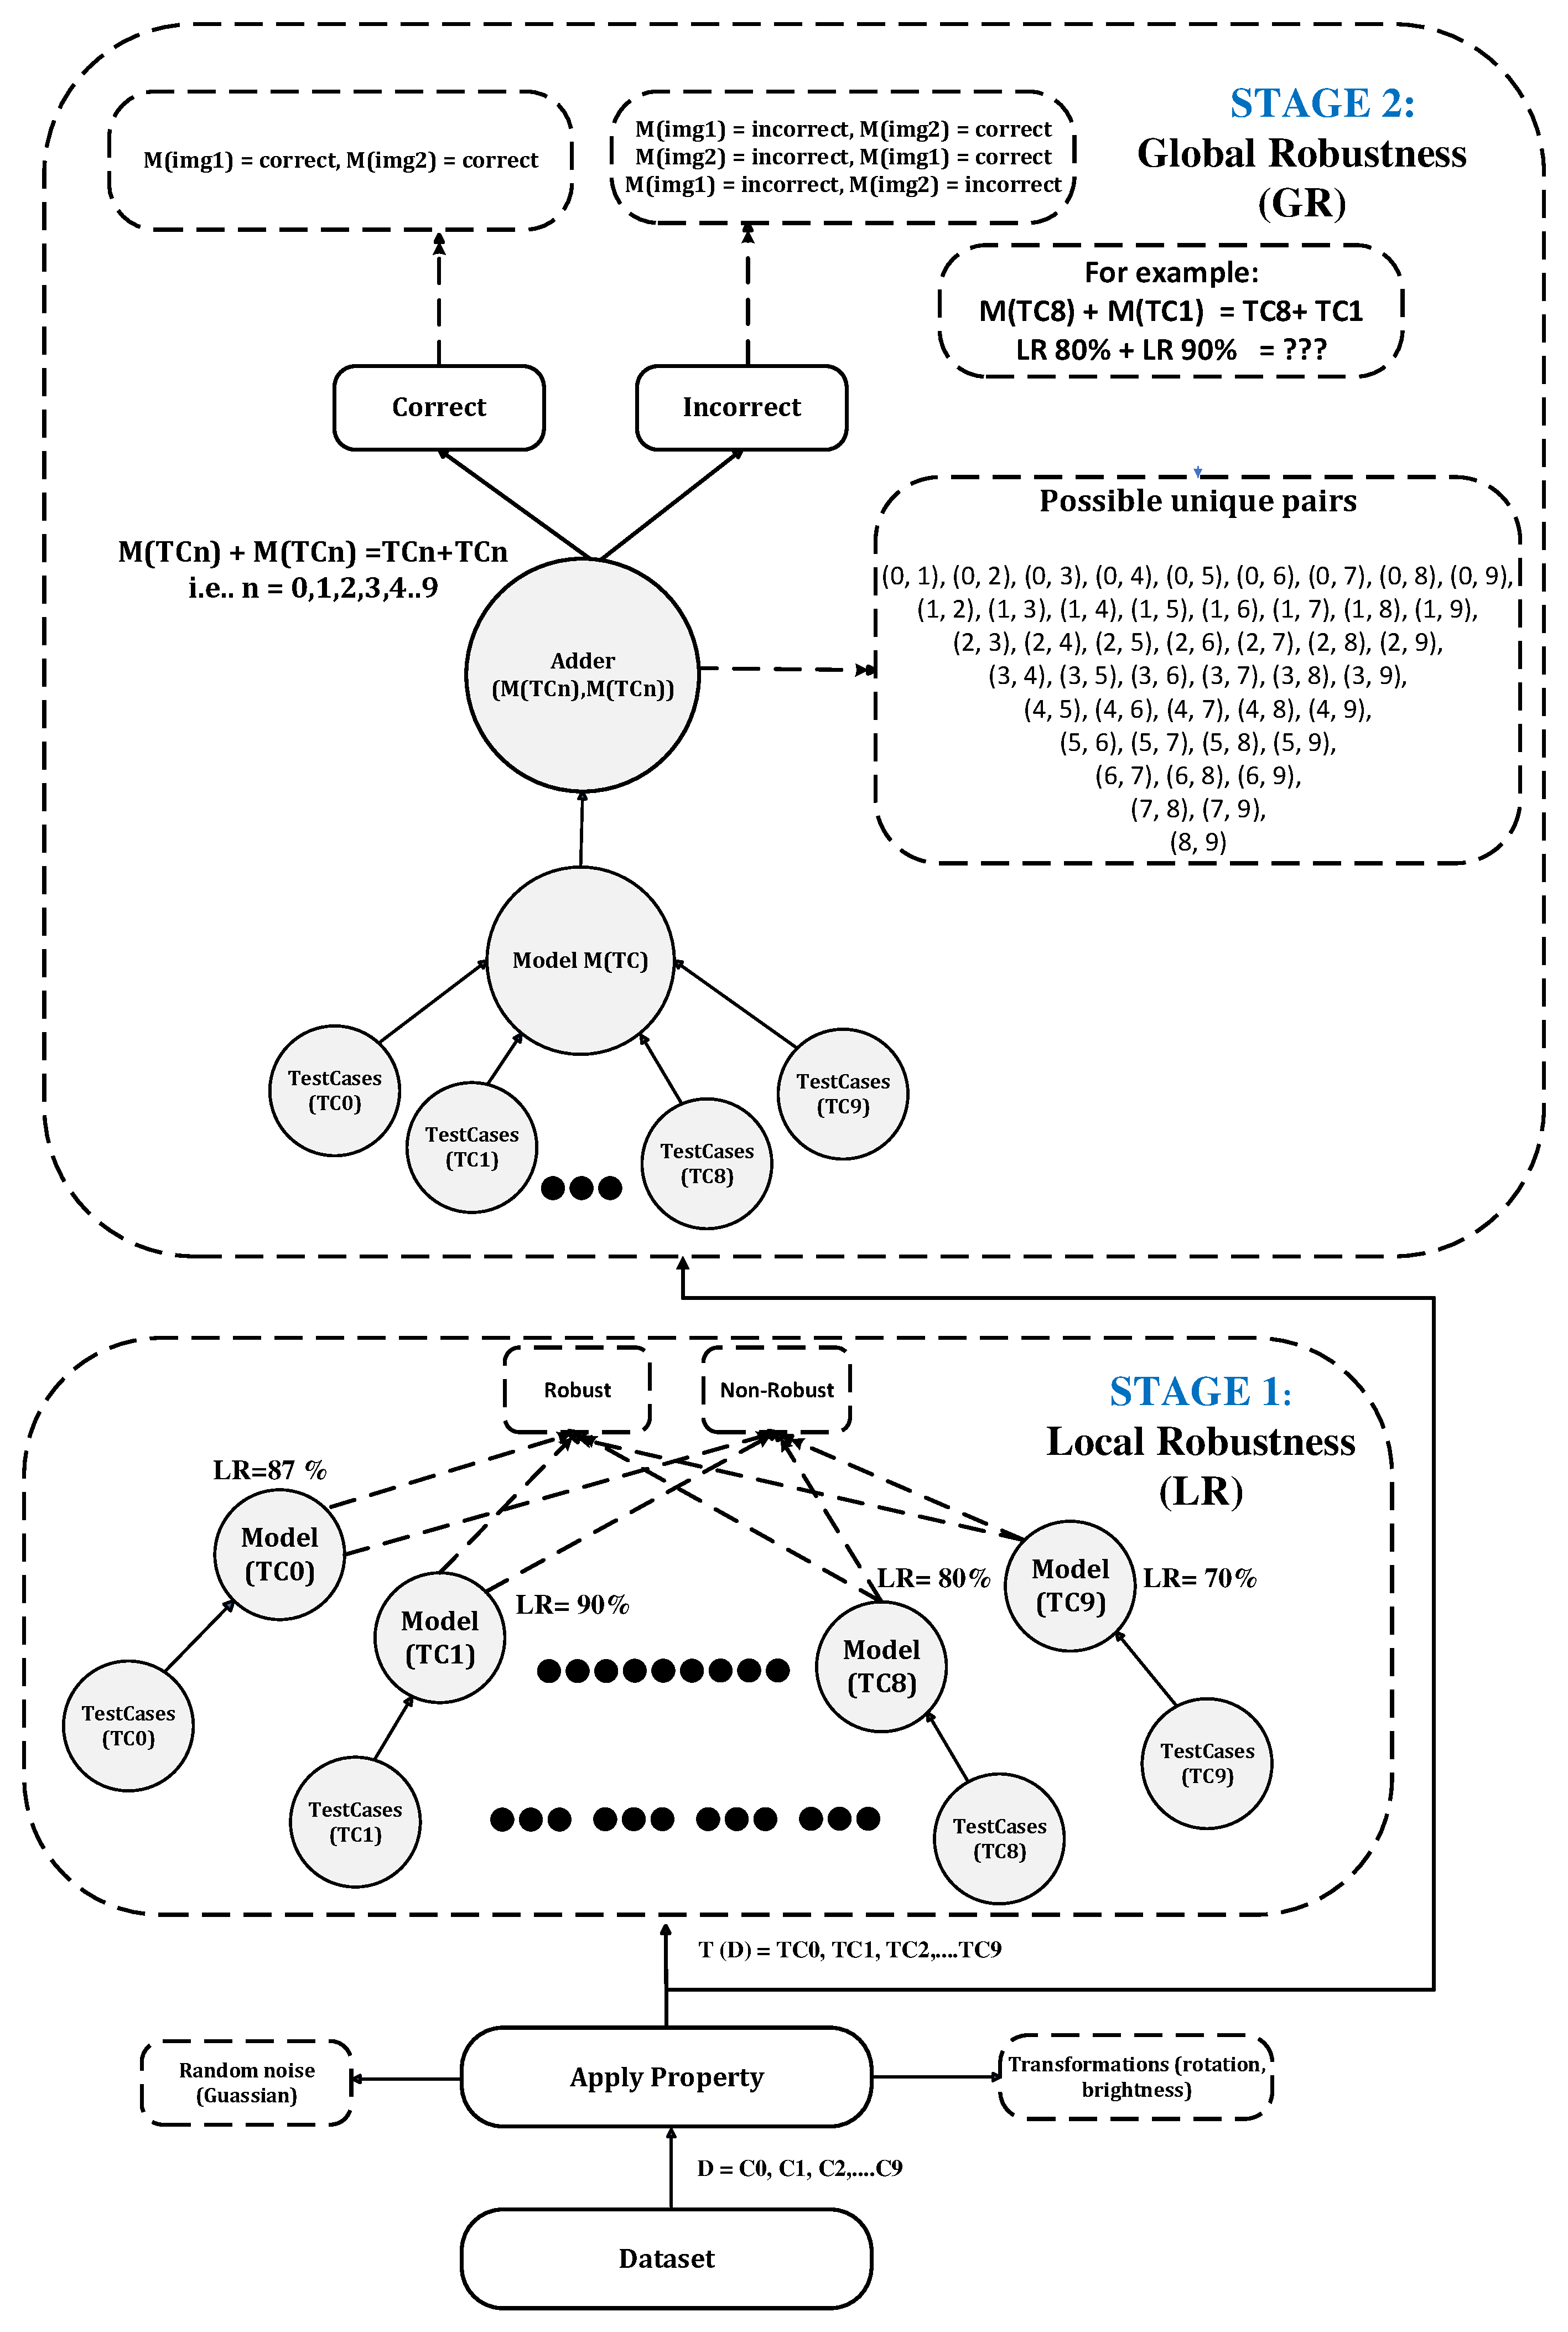
\includegraphics[width=\linewidth]{paper_images/addermodelview.pdf}
    \caption{Graphical Representation}
    \label{fig:graph}
\end{figure*}
\section{Research Questions}
\begin{itemize}[noitemsep]
    \item How to specify relevant local robustness properties?
    \item Can probabilistic graphical models effectively assess local and global robustness in deep learning?
\end{itemize}

\section{Experimental Setup}
% Your content here

\section{Threats to Validity}
\begin{itemize}[noitemsep]
    \item Assume random samples
    \item Valid test case generation
\end{itemize}

\section{Related Work}
% Your content here

\section{Conclusion}
% Your conclusion here

\begin{thebibliography}{01}
    \bibitem{Saad} Reference details
\end{thebibliography}

\end{document}
